\documentclass[12pt,a4paper]{article}

% ---------- Codificação e idioma ----------
\usepackage[T1]{fontenc}
\usepackage[utf8]{inputenc}
\usepackage[brazilian]{babel}
\usepackage{lmodern}
\usepackage{textcomp}
\usepackage{enumitem}

% ---------- Layout de página (medido no template oficial) ----------
\usepackage[a4paper,left=3cm,right=2cm,top=2cm,bottom=2cm,headheight=14pt,headsep=0.6cm,includeheadfoot]{geometry}
\usepackage{setspace}
\usepackage{indentfirst}
\setstretch{1.5}
\setlength{\parindent}{1.25cm}

% ---------- Cabeçalho e rodapé ----------
\usepackage{fancyhdr}
\pagestyle{fancy}
\fancyhf{}
\renewcommand{\headrulewidth}{0.4pt}
\renewcommand{\footrulewidth}{0pt}
\fancyhead[L]{\small Usabilidade e Inclusão Digital: um Estudo sobre as Dificuldades de Pessoas Acima de 45 Anos no Uso de \textit{E-commerce}}
\fancyfoot[C]{\thepage}
\fancypagestyle{firstpage}{%
  \fancyhf{}
  \renewcommand{\headrulewidth}{0pt}
  \fancyfoot[C]{\thepage}
}

% ---------- Tabelas e figuras ----------
\usepackage{graphicx}
\usepackage{array}
\usepackage{booktabs}
\usepackage{longtable}

% ---------- Seções (numeração manual via \setcounter, estilo igual ao template) ----------
\usepackage{titlesec}
\titleformat{\section}{\normalfont\bfseries}{\thesection}{0.6em}{}
\titleformat{\subsection}{\normalfont\bfseries}{\thesubsection}{0.6em}{}
\titleformat{\subsubsection}{\normalfont\bfseries\itshape}{\thesubsubsection}{0.6em}{}
\titlespacing*{\section}{0pt}{18pt}{8pt}
\titlespacing*{\subsection}{0pt}{14pt}{6pt}
\titlespacing*{\subsubsection}{0pt}{12pt}{6pt}

% ---------- Links ----------
\usepackage[colorlinks=true, linkcolor=black, urlcolor=blue, citecolor=black]{hyperref}
\usepackage{xurl}

% ---------- Referências bibliográficas no padrão ABNT (via abntex2cite) ----------
\usepackage[alf]{abntex2cite}
\renewcommand{\refname}{REFERÊNCIAS}

\begin{document}
\citeoption{abnt-nbr10520=1988}
\thispagestyle{firstpage}

% ================= CABEÇALHO INSTITUCIONAL =================
\begin{center}

\includegraphics[width=4.5cm]{figuras/logo_puc.png}\\[0.15cm]
{\normalsize PONTIFÍCIA UNIVERSIDADE CATÓLICA DE MINAS GERAIS}\\
{\normalsize Instituto de Ciências Exatas e de Informática}
\end{center}

\vspace{0.3cm}

% ================= TÍTULO =================
\renewcommand{\thefootnote}{\fnsymbol{footnote}}
\noindent{\Large Usabilidade e Inclusão Digital: um Estudo sobre as Dificuldades de Pessoas Acima de 45 Anos no Uso de \textit{E-commerce}\footnote{Artigo apresentado ao Instituto de Ciências Exatas e Informática da Pontifícia Universidade Católica de Minas Gerais, campus Betim, como pré-requisito parcial para obtenção do título de Bacharel em Sistemas de Informação.}}

\vspace{0.6cm}

% ================= AUTORES =================
\renewcommand{\thefootnote}{\arabic{footnote}}
\setcounter{footnote}{0}
\begin{flushright}
Tiago Rafael Martins Cardoso\footnote{Aluno(a) do Programa de Graduação em Sistemas de Informação -- \url{tiago.@sga.pucminas.br}.}\\
Victoria Gonçalves da Silva\footnote{Aluno(a) do Programa de Graduação em Sistemas de Informação -- \url{Victoria.silva.1464849@sga.pucminas.br}.}\\
Juliana Santiago Teixeira\footnote{Professor(a) do Programa de Graduação em Sistemas de Informação.}
\end{flushright}

\vspace{0.5cm}

% ================= RESUMO (espaçamento simples, conforme NBR 6028) =================
\begin{spacing}{1.0}
\begin{center}
\textbf{Resumo}
\end{center}
\noindent O crescimento do \textit{e-commerce} no Brasil intensificou a necessidade de interfaces acessíveis para públicos diversos, incluindo pessoas acima de 45 anos, que ainda enfrentam barreiras cognitivas, visuais e de navegação ao realizar compras on-line. Investigar essas dificuldades torna-se essencial para promover inclusão digital e aprimorar a experiência de uso, alinhando o desenvolvimento às heurísticas de usabilidade e às diretrizes de acessibilidade. Nesse contexto, o objetivo deste estudo é avaliar o impacto de melhorias de design na eficiência, eficácia e satisfação desses usuários ao utilizarem uma plataforma de \textit{e-commerce}. Como contribuição, a pesquisa apresenta um protótipo otimizado e evidências empíricas que demonstram como diretrizes de usabilidade e acessibilidade podem reduzir barreiras e melhorar a jornada de compra desse público.

\noindent\textbf{Palavras-chave:} Usabilidade; Acessibilidade digital; \textit{E-commerce}; Inclusão digital; Usuários acima de 45 anos.
\end{spacing}

\vspace{0.6cm}

% ================= 1. INTRODUÇÃO =================
\section{INTRODUÇÃO}

O comércio eletrônico (\textit{e-commerce}) surgiu no final da década de 1970, com o britânico Michael Aldrich, pioneiro ao conectar uma televisão a um computador para realizar transações comerciais, marco inicial das compras on-line \cite{telegraph2014}. No Brasil, o setor cresceu de forma significativa e, em 2023, atingiu R\$ 254,4 bilhões em faturamento, consolidando-se como o segundo maior canal de vendas do varejo nacional, atrás apenas do autosserviço \cite{nielseniq2024}.

Paralelamente, o envelhecimento populacional tem se acelerado: mais da metade dos brasileiros (56,1\%) possui 30 anos ou mais, com destaque para o aumento de pessoas acima de 45 anos \cite{ibge2022}. Diante desse cenário, a usabilidade torna-se essencial. Como destaca \citeonline{nielsen1993}, sistemas devem equilibrar facilidade de aprendizado e eficiência conforme o nível de experiência do usuário. Assim, é fundamental desenvolver interfaces acessíveis e intuitivas, especialmente para o público mais velho, garantindo inclusão digital e participação social \cite{rodriguessantos2022}. A exclusão digital representa um desafio crescente na era das tecnologias da informação e comunicação, pois, embora o ciberespaço tenha ampliado o acesso à cultura, à política e ao mercado, muitos grupos ainda permanecem à margem desse ambiente \cite{moreira2023}. No contexto do \textit{e-commerce}, essa exclusão se manifesta em barreiras de acesso e usabilidade, especialmente entre os consumidores mais velhos, que enfrentam dificuldades para compreender e utilizar as interfaces digitais \cite{cetic2024}. O estudo Conectividade Significativa aponta que 61\% das pessoas com 60 anos ou mais possuem baixa conectividade, reflexo da desigualdade educacional e socioeconômica.

Diante desse cenário, torna-se necessário questionar: como um conjunto de otimizações de design, baseado em heurísticas de usabilidade, impacta a eficácia, eficiência e satisfação de usuários acima de 45 anos durante sua jornada em um site de \textit{e-commerce} brasileiro?

A pesquisa é relevante por suas dimensões sociais, mercadológicas e científicas, ao investigar a inclusão digital de indivíduos com mais de 45 anos, faixa etária crescente no Brasil \cite{ibge2022}. O estudo destaca como o envelhecimento pode afetar o uso de tecnologias digitais e a necessidade de interfaces acessíveis, promovendo autonomia, participação social e econômica. A justificativa da hipótese apoia-se em fundamentos consolidados com base em princípios de Interação Humano-Computador, como as Heurísticas de \citeonline{nielsen1993} e as Diretrizes de Acessibilidade da W3C, a pesquisa busca preencher a lacuna científica existente sobre a eficácia dessas práticas em contextos culturais e tecnológicos específicos, avaliando como otimizações de design podem melhorar a experiência de compra online para esse público.

O objetivo geral deste trabalho é avaliar a eficácia de um conjunto de diretrizes de design, focadas em acessibilidade e usabilidade, na otimização da experiência de compra online para usuários com mais de 45 anos. Já os objetivos específicos são:

\begin{enumerate}[label=\roman*)]
    \item Caracterizar os principais desafios de interação e as barreiras de acessibilidade que comprometem a jornada de compra online do público-alvo em um site de \textit{e-commerce} de referência;
    \item Estruturar um conjunto de melhorias de design de interface e experiência do usuário (UI/UX) com base nos problemas diagnosticados e na literatura da área;
    \item Validar o impacto das melhorias propostas na eficiência, eficácia e satisfação dos usuários, por meio de testes comparativos entre a interface original e o protótipo desenvolvido.
\end{enumerate}

Este texto está estruturado em seis seções. A seção 2 apresenta o referencial teórico, abordando conceitos de usabilidade, acessibilidade e inclusão digital. A seção 3 descreve os trabalhos relacionados que tratam de estudos semelhantes ao tema. Na seção 4 é apresentada a metodologia utilizada, com as etapas e o ambiente de desenvolvimento. A seção 5 detalha o desenvolvimento do sistema e os testes realizados. Por último, a seção 6 apresenta a conclusão, com a discussão dos resultados, contribuições e sugestões para trabalhos futuros.

% ================= 2. REFERENCIAL TEÓRICO =================
\section{REFERENCIAL TEÓRICO}

O referencial teórico é organizado em forma de pirâmide, inicia com os conceitos gerais de usabilidade, passa pela acessibilidade digital e finaliza com a inclusão digital de pessoas acima de 45 anos. Essa estrutura ajuda a conectar a base teórica às dificuldades desse público no uso de \textit{e-commerce}.

\subsection{Usabilidade}

Segundo o autor Jakob Nielsen, ``usabilidade é um atributo de qualidade que avalia o quão fácil é para um usuário interagir com um sistema'' (Nielsen, 1993, p. 26, tradução nossa). O autor define cinco componentes essenciais: facilidade de aprendizado (\textit{learnability}), eficiência de uso (\textit{efficiency}), facilidade de memorização (\textit{memorability}), baixo índice de erros (\textit{errors}) e satisfação subjetiva (\textit{satisfaction}). Esses fatores permitem avaliar a experiência do usuário de forma objetiva e mensurável, auxiliando no desenvolvimento de sistemas mais intuitivos.

\citeonline{norman1988}, complementa esse entendimento ao afirmar que o design deve ser centrado no usuário, considerando suas limitações cognitivas e motoras. Norman argumenta que produtos e interfaces bem projetados tornam as ações compreensíveis e as respostas previsíveis, permitindo ao usuário compreender a relação entre sua ação e o resultado obtido. Ele introduz conceitos fundamentais como \textit{affordance} e \textit{feedback}, que ajudam o usuário a entender o que é possível fazer em uma interface.

\citeonline{krug2013} reforça esses princípios ao sintetizar a ideia central de usabilidade com seu famoso lema: ``\textit{Don't make me think}'' (``Não me faça pensar''). No primeiro capítulo de seu livro homônimo, Krug defende que o melhor design é aquele que reduz o esforço cognitivo do usuário, tornando a navegação e a compreensão do conteúdo quase automáticas. Para o autor, quando o usuário precisa parar e pensar sobre como usar um site, há um problema de design. Portanto, a simplicidade e a clareza são pilares para uma boa experiência digital, especialmente em ambientes como o \textit{e-commerce}, onde decisões rápidas e intuitivas são essenciais.

\subsection{Acessibilidade digital}

A discussão sobre acessibilidade digital está fortemente ligada à visão de \citeonline{bernerslee1997}, criador da World Wide Web. Em sua obra \textit{Weaving the Web}, Berners-Lee destaca que o poder da Web está em sua universalidade. O acesso por todas as pessoas, independentemente de deficiência, é um aspecto essencial. Essa afirmação tornou-se a base para as iniciativas de acessibilidade desenvolvidas pelo World Wide Web Consortium (W3C), organização responsável pela criação e manutenção dos padrões da web.

Dentro do W3C, a Web Accessibility Initiative (WAI) desenvolve as Diretrizes de Acessibilidade para Conteúdo Web (WCAG), que orientam a criação de sites acessíveis. Essas diretrizes baseiam-se em quatro princípios fundamentais: perceptível, operável, compreensível e robusto. Cada princípio define critérios mensuráveis que ajudam desenvolvedores e designers a construírem interfaces que possam ser utilizadas por todos os públicos, inclusive pessoas idosas ou com deficiência visual, auditiva ou cognitiva.

\citeonline{horton2014}, em \textit{A Web for Everyone}, reforçam que projetar para acessibilidade não é apenas atender a um público específico, mas criar experiências melhores para todos. Segundo as autoras, o design inclusivo resulta em produtos mais fáceis, úteis e agradáveis para todos os usuários. Elas argumentam que boas práticas de acessibilidade como contraste adequado, tipografia legível e navegação simplificada, beneficiam toda a população, não apenas pessoas com limitações. Assim, acessibilidade e usabilidade são dimensões complementares do design digital.

\subsection{Inclusão digital de pessoas acima de 45 anos}

A inclusão digital é uma das dimensões mais importantes da sociedade contemporânea, conforme discute Castells em \textit{A Sociedade em Rede} \cite{castells1999}. O autor explica que vivemos em uma ``era da informação'', na qual o acesso e o uso das tecnologias digitais se tornaram determinantes para a participação social, econômica e cultural. Castells destaca que a exclusão tecnológica cria novas formas de desigualdade, reforçando a divisão entre os que têm acesso à informação e os que permanecem desconectados.

\citeonline{levy1999}, em \textit{Cibercultura}, amplia essa discussão ao afirmar que a internet possibilita a formação de uma ``inteligência coletiva'', na qual o conhecimento é compartilhado e expandido pela colaboração em rede. No entanto, o autor também alerta que esse potencial não se concretiza igualmente para todos: os indivíduos que não possuem familiaridade tecnológica ou acesso adequado acabam excluídos do processo de construção coletiva do saber.

Por sua vez, \citeonline{livingstone2013}, em \textit{Children and the Internet: A Global Study of Digital In/Exclusion}, observa que a exclusão digital vai além da ausência de dispositivos ou conexão. Ela envolve também fatores sociais, culturais e psicológicos que influenciam a forma como as pessoas se apropriam da tecnologia. Embora seu estudo seja voltado ao público jovem, a autora mostra que a inclusão digital exige mais do que infraestrutura, requer também competências e confiança no uso. Essa perspectiva pode ser aplicada à análise das dificuldades enfrentadas por pessoas com mais de 45 anos no uso do \textit{e-commerce}, que muitas vezes enfrentam barreiras cognitivas e de design que limitam sua autonomia online.

Diante disso, a inclusão digital também depende da forma como as tecnologias são projetadas e disponibilizadas aos usuários. Nesse sentido, a usabilidade das plataformas de comércio eletrônico assume um papel fundamental para favorecer a participação autônoma de pessoas acima de 45 anos nas compras online. Conforme os princípios de usabilidade apresentados por \citeonline{nielsen1993} e \citeonline{krug2013}, as interfaces devem facilitar a compreensão das ações, orientar os usuários durante a navegação e reduzir o esforço necessário para realizar tarefas. Assim, a aplicação desses princípios ao \textit{e-commerce} pode contribuir para minimizar as dificuldades de uso, reduzir erros e aumentar a confiança dos usuários. Dessa forma, a usabilidade deixa de ser apenas uma característica técnica das plataformas e passa a representar um elemento importante para a inclusão digital, especialmente para pessoas acima de 45 anos que enfrentam dificuldades na utilização de serviços de comércio eletrônico.

% ================= 3. TRABALHOS RELACIONADOS =================
\section{TRABALHOS RELACIONADOS}

\citeonline{tilvitz2022} investigaram a inclusão digital de idosos e o uso do \textit{smartphone} como principal meio de interação tecnológica. A pesquisa, de caráter quantitativo, foi aplicada a cem pessoas acima de sessenta anos e analisada com o software SPSS, identificando as dificuldades e sentimentos relacionados ao uso de dispositivos móveis. As autoras destacam que, apesar do interesse dos idosos em participar do mundo digital, persistem barreiras cognitivas e de design nas interfaces. Assim como neste trabalho, as autoras reconhecem a necessidade de otimizar a usabilidade para favorecer a adaptação dos usuários mais velhos; entretanto, diferentemente da proposta atual, o estudo foca no uso geral de smartphones, e não especificamente em plataformas de \textit{e-commerce}.

\citeonline{vasconcelos2021} realizaram uma revisão sistemática sobre usabilidade em aplicativos móveis voltados para idosos, buscando identificar critérios de design que promovam acessibilidade e satisfação no uso. Os autores observaram que as heurísticas mais aplicadas envolvem aspectos visuais, legibilidade e feedbacks claros. Assim como o presente estudo, o artigo reforça a importância da usabilidade e das heurísticas de \citeonline{nielsen1993} para o desenvolvimento de interfaces acessíveis. No entanto, a pesquisa deles é de natureza bibliográfica, enquanto este trabalho aplica as diretrizes em um contexto prático de \textit{e-commerce}, com foco em testes empíricos com usuários.

\citeonline{silvasiqueiradezani2023} conduziram um estudo exploratório sobre a acessibilidade digital nas quatro maiores plataformas de \textit{marketplace} do Brasil, visando identificar barreiras para pessoas com deficiência visual. Utilizando ferramentas de validação automática, como o AChecker e os validadores da W3C, os autores analisaram a conformidade dos sites com as diretrizes WCAG nos níveis A, AA e AAA. Os resultados revelaram que todas as plataformas apresentaram erros de validação, sendo que o Magazine Luiza obteve o melhor desempenho em conformidade, enquanto Amazon e Mercado Livre apresentaram maiores desafios nos níveis mais avançados de acessibilidade. Este trabalho correlaciona-se com a presente pesquisa ao investigar a inclusão em grandes \textit{e-commerces}; contudo, distingue-se por adotar uma metodologia baseada exclusivamente em validadores automáticos de código, enquanto esta proposta foca na experiência de uso sob a ótica do envelhecimento (pessoas acima de 45 anos) e na aplicação prática de testes de usabilidade.

\citeonline{rodrigues2022} analisou a usabilidade de aplicativos bancários móveis (\textit{Internet Banking}) para o público idoso, por meio de testes com participantes entre 60 e 80 anos. O estudo revelou que a principal barreira não está apenas nas limitações cognitivas, mas também no receio de cometer erros em operações financeiras, o que reduz a confiança no uso. A pesquisa contribui com evidências empíricas relevantes, especialmente ao mostrar como a insegurança e o design complexo afetam a experiência de pessoas idosas. Embora compartilhe o mesmo público-alvo, a presente pesquisa se diferencia por abordar plataformas de compra on-line, ampliando o escopo para interações de consumo digital.

Por fim, \citeonline{silva2024} discutiu o uso do aplicativo governamental SouGov por idosos, relacionando os desafios de acessibilidade, limitações cognitivas e falta de design inclusivo. A autora propôs soluções baseadas em design universal, capacitação digital e políticas públicas de inclusão. Seu trabalho se aproxima da presente proposta ao defender que a acessibilidade tecnológica é um fator essencial de cidadania digital. No entanto, enquanto Silva enfatiza o papel do governo e das políticas de inclusão, o presente estudo concentra-se na experiência de usabilidade em ambientes comerciais digitais.

% ================= 4. METODOLOGIA =================
\section{METODOLOGIA}

Este trabalho adotou uma abordagem aplicada e experimental, com foco no desenvolvimento e avaliação de uma solução tecnológica voltada à melhoria da experiência de uso de plataformas de comércio eletrônico por indivíduos com idade entre 45 e 60 anos. A metodologia foi estruturada de forma a permitir a comparação da experiência do usuário entre uma plataforma de \textit{e-commerce} de referência (Amazon) e o protótipo desenvolvido, buscando assegurar rigor metodológico e confiabilidade nos resultados obtidos.

Para a coleta e análise dos dados, foram utilizados instrumentos predominantemente quantitativos, por meio de questionários estruturados com categorias de dificuldade pré-definidas, complementados por um componente qualitativo. Sempre que o participante selecionava a opção ``Outra dificuldade'', um campo de texto livre era apresentado para o relato detalhado da experiência, permitindo identificar problemas não previstos nas categorias fechadas.

\subsection{Classificação da pesquisa}

Quanto à sua natureza, esta pesquisa foi classificada como aplicada, pois buscou solucionar um problema prático relacionado à usabilidade e acessibilidade em plataformas de \textit{e-commerce}.

Em relação à abordagem, caracterizou-se como mista (quantitativa e qualitativa), predominantemente quantitativa: as respostas às tarefas foram coletadas por meio de questões de múltipla escolha com taxonomias de dificuldade pré-categorizadas (por exemplo, dificuldade para localizar o botão de login, confusão entre ``Adicionar ao carrinho'' e ``Comprar agora'', excesso de informações na tela, entre outras), permitindo tratamento estatístico direto das respostas. O componente qualitativo foi preservado pelo campo de texto condicional associado à opção ``Outra dificuldade'', que permitiu registrar relatos livres não antecipados pelas categorias fechadas.

Do ponto de vista dos objetivos, a pesquisa caracterizou-se como descritiva, pois buscou identificar e descrever as principais dificuldades de interação enfrentadas por pessoas entre 45 e 60 anos durante a utilização de uma plataforma de comércio eletrônico, além de avaliar os resultados associados às melhorias implementadas no protótipo. A comparação entre as duas interfaces permitiu analisar diferenças na execução das tarefas, na ocorrência de dificuldades e na percepção de facilidade de uso dos participantes.

Quanto aos procedimentos técnicos, a pesquisa apresentou caráter experimental, uma vez que envolveu o desenvolvimento de um protótipo com melhorias de usabilidade e acessibilidade e a comparação de sua utilização com uma plataforma de referência. Essa comparação buscou verificar possíveis diferenças no desempenho e na experiência dos participantes após a implementação das melhorias propostas.

\subsection{Participantes}

O público-alvo da pesquisa foi composto por pessoas com idade entre 45 e 60 anos, categorizadas em três faixas etárias para fins de caracterização da amostra: 45 a 50 anos, 51 a 55 anos e 56 a 60 anos. A pesquisa obteve uma amostra de 55 respostas ao questionário de usabilidade, utilizado para investigar as experiências, dificuldades e percepções dos participantes durante a utilização de plataformas de comércio eletrônico.

O recrutamento dos participantes ocorreu por meio de compartilhamento do link do questionário pelo WhatsApp, com participação voluntária. Como critérios de inclusão, foram considerados indivíduos com idade entre 45 e 60 anos que aceitaram participar da pesquisa e responderam às questões propostas. Para a análise dos resultados, foram consideradas as respostas que atenderam aos critérios estabelecidos para o estudo.

Antes da realização das atividades, foi coletado um perfil inicial dos participantes, contemplando informações sobre idade, experiência prévia com compras pela internet, frequência de utilização de sites ou aplicativos de compra e familiaridade com a plataforma avaliada. Esse levantamento permitiu caracterizar a amostra e considerar a experiência prévia dos participantes na interpretação dos resultados obtidos.

\subsection{Etapas da pesquisa}

O desenvolvimento do trabalho foi dividido nas seguintes etapas:

\begin{enumerate}[label=\alph*)]
    \item levantamento de requisitos e definição da plataforma de referência (Amazon);
    \item elaboração do questionário estruturado de teste de usabilidade;
    \item aplicação do questionário na plataforma de referência (Amazon);
    \item modelagem das soluções de design com base nas dificuldades identificadas;
    \item desenvolvimento do protótipo de \textit{e-commerce} acessível;
    \item aplicação do mesmo questionário no protótipo desenvolvido;
    \item análise comparativa dos resultados entre a plataforma de referência e o protótipo.
\end{enumerate}

Inicialmente, foi conduzido um levantamento bibliográfico sobre acessibilidade digital, usabilidade, experiência do usuário e inclusão de adultos entre 45 e 60 anos no ambiente virtual. Em seguida, definiu-se a Amazon como plataforma de \textit{e-commerce} de referência para a primeira rodada de testes, por se tratar de uma das maiores e mais utilizadas plataformas do setor.

O instrumento de coleta foi estruturado em um questionário aplicado via Google Forms, organizado da seguinte forma: (i) bloco de perfil do participante (idade, experiência prévia com compras on-line, frequência de uso e familiaridade com a plataforma avaliada); (ii) cinco tarefas sequenciais representativas de uma jornada de compra --- realizar login, pesquisar um produto, adicionar um produto ao carrinho, remover um produto do carrinho e concluir a compra --- cada uma acompanhada de uma questão sobre o sucesso da tarefa (``Sim, sem dificuldades'' / ``Sim, mas tive dificuldades'' / ``Não consegui realizar'') e de uma questão de múltipla escolha com as principais categorias de dificuldade associadas àquela tarefa; (iii) uma estimativa percebida do tempo total gasto para concluir as tarefas, também em formato de múltipla escolha; e (iv) uma avaliação geral da plataforma, incluindo a maior dificuldade encontrada, a tarefa considerada mais fácil, a necessidade de ajuda durante o teste e a percepção geral de facilidade de uso.

Paralelamente à aplicação do questionário, foi realizada a observação direta dos participantes durante a execução das tarefas, com registro do tempo real de execução de cada tarefa, do número de erros e da necessidade de auxílio, por meio de uma planilha de observação preenchida pelo pesquisador. Esse registro permitiu comparar o tempo percebido pelos participantes informado no questionário, com o tempo efetivamente medido, evidenciando eventuais discrepâncias entre percepção e desempenho real.

Com base nas dificuldades relatadas e observadas na plataforma de referência, foram estabelecidas diretrizes de design e funcionalidades alinhadas às heurísticas de \citeonline{nielsen1993} e às recomendações da WCAG 2.1 \cite{w3cwcag2018}, que orientaram o desenvolvimento do protótipo em aspectos como legibilidade, contraste, navegação simplificada e linguagem clara.

Com as diretrizes definidas, foi desenvolvido o protótipo de \textit{e-commerce}, abrangendo a estrutura de navegação, o layout visual, a categorização de produtos e o fluxo completo de compra, com foco em acessibilidade.

Após a implementação, os mesmos participantes foram convidados a repetir as cinco tarefas no protótipo desenvolvido, respondendo ao mesmo instrumento de coleta aplicado na etapa anterior. Essa simetria entre os dois instrumentos --- idênticos em estrutura e categorias de resposta --- permitiu a comparação estatística direta entre a plataforma de referência e o protótipo.

Por fim, os dados provenientes das duas rodadas de aplicação (Amazon e protótipo) foram comparados sistematicamente na ferramenta Microsoft Excel, possibilitando analisar o impacto das melhorias implementadas e confirmar se os objetivos propostos pelo estudo foram alcançados.

\bigskip
\begin{center}
\begin{minipage}{\textwidth}
\centering
\textbf{Figura 1 -- Fluxograma das etapas da pesquisa}\\[0.3cm]
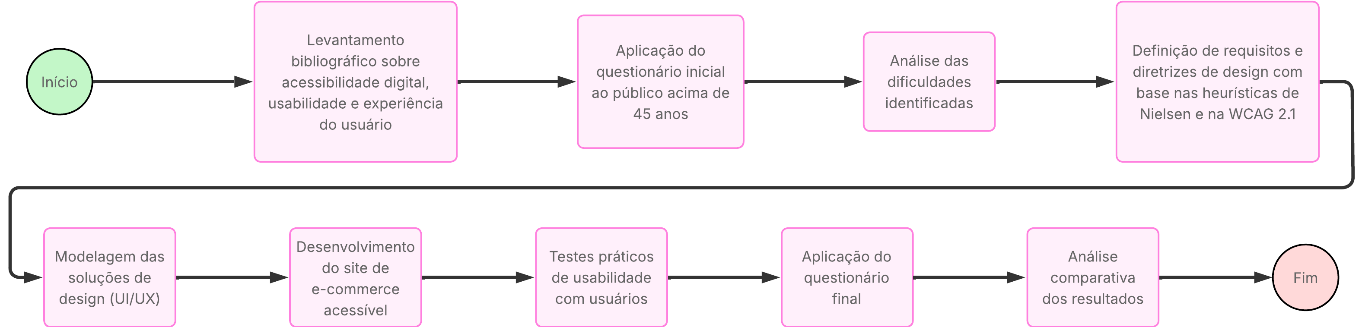
\includegraphics[width=\textwidth]{figuras/fluxograma.png}\\[0.2cm]
{\small\textbf{Fonte: Elaborada pelo autor}}
\end{minipage}
\end{center}
\bigskip

\subsection{Ambiente de desenvolvimento}

O ambiente de desenvolvimento utilizado neste trabalho foi estruturado para permitir a criação de um protótipo funcional de \textit{e-commerce} acessível, alinhado às diretrizes de usabilidade de \citeonline{nielsen1993} e às recomendações da WCAG 2.1 \cite{w3cwcag2018}. O Quadro 1 apresenta as ferramentas adotadas, organizadas por funcionalidade.

\begin{center}
\textbf{Quadro 1 -- Ferramentas do ambiente de desenvolvimento}
\end{center}
\begin{center}
\begin{tabular}{|p{5.4cm}|p{5.4cm}|}
\hline
\textbf{Funcionalidade} & \textbf{Ferramenta} \\
\hline
Prototipação e Design (UI/UX) & Figma \\
\hline
Front-end & HTML5, CSS3 e JavaScript \\
\hline
Back-end & Node.js com Express \\
\hline
Banco de Dados & PostgreSQL \\
\hline
Controle de Versão & Git + GitHub \\
\hline
Ambiente de Programação & Visual Studio Code (VS Code) \\
\hline
Levantamento de dados & Google Forms \\
\hline
Análise de Dados & Microsoft Excel \\
\hline
\end{tabular}
\end{center}
\begin{center}
{\small\textbf{Fonte: Elaborado pelo autor}}
\end{center}

% ================= 5. METODOLOGIA =================
\section{DESENVOLVIMENTO E RESULTADOS}

\subsection{Caracterização dos participantes}

A pesquisa obteve 55 respostas ao questionário de usabilidade, com o objetivo de investigar as experiências e dificuldades de pessoas entre 45 e 60 anos durante a utilização de plataformas de comércio eletrônico.

Quanto à faixa etária, 50,9\% dos participantes tinham entre 45 e 50 anos, 23,6\% entre 51 e 55 anos e 25,5\% entre 56 e 60 anos. Em relação à experiência com compras on-line, 94,5\% afirmaram já ter realizado esse tipo de compra. Além disso, 54,5\% utilizavam plataformas de comércio eletrônico recorrentemente e 30,9\% algumas vezes. Esses resultados demonstraram que a maioria dos participantes já possuía experiência com compras pela internet, embora apresentasse diferentes níveis de familiaridade com as plataformas avaliadas.

\subsection{Resultados da avaliação da Amazon}

A avaliação da Amazon contemplou cinco tarefas: realizar login, pesquisar produtos, adicionar e remover itens do carrinho e concluir a compra.

No login, 69,8\% dos participantes realizaram a tarefa sem dificuldades, enquanto 17,0\% não conseguiram concluí-la. Na pesquisa de produtos, 69,8\% não encontraram dificuldades e 13,2\% não conseguiram realizar a atividade. A inclusão de produtos no carrinho apresentou o melhor resultado, com 77,4\% de execução sem dificuldades. Na remoção de itens, esse percentual foi de 75,5\%. Já na conclusão da compra, 73,6\% realizaram a tarefa sem dificuldades, enquanto 18,9\% não conseguiram concluí-la.

Na avaliação geral, 61,5\% classificaram a Amazon como fácil de utilizar, e 69,8\% afirmaram ter realizado todas as tarefas sem ajuda. Apesar da percepção predominantemente favorável, os resultados evidenciaram dificuldades principalmente no login e na conclusão da compra.

\subsection{Resultados da avaliação da Shopee}

Na Shopee, também foram avaliadas as cinco tarefas relacionadas à jornada de compra.

No login, 74,5\% dos participantes realizaram a tarefa sem dificuldades, enquanto 16,4\% não conseguiram concluí-la. Na pesquisa de produtos, 72,7\% não encontraram dificuldades e 9,1\% não conseguiram realizar a atividade. Na inclusão de produtos no carrinho, 77,8\% realizaram a tarefa sem dificuldades. Na remoção de itens, esse percentual foi de 76,4\%. Na conclusão da compra, 77,8\% conseguiram realizar a tarefa sem dificuldades, enquanto 14,8\% não conseguiram concluí-la.

Na avaliação geral, 63,6\% consideraram a Shopee fácil de utilizar, e 77,4\% afirmaram ter realizado todas as tarefas sem ajuda. Embora os resultados tenham sido favoráveis, ainda foram identificadas dificuldades relacionadas ao login, à navegação e à finalização da compra.

\subsection{Análise comparativa dos resultados}

Figura 2 – Caracterização dos participantes e avaliação da usabilidade das plataformas Amazon e Shopee (COLOCAR A IMAGEM)

A comparação descritiva demonstrou que a maioria dos participantes conseguiu realizar as tarefas sem dificuldades nas duas plataformas. Na Amazon, os percentuais variaram de 69,8\% a 77,4\%, enquanto, na Shopee, variaram de 72,7\% a 77,8\%. A Shopee apresentou percentuais ligeiramente superiores na avaliação geral de facilidade de uso (63,6\%, contra 61,5\% na Amazon) e na realização das tarefas sem ajuda (77,4\%, contra 69,8\%).

Entretanto, esses resultados não permitem concluir isoladamente que uma plataforma apresentou usabilidade superior à outra, pois a familiaridade prévia dos participantes com cada ambiente pode ter influenciado as respostas. De modo geral, os dados evidenciaram a importância de interfaces claras, navegação intuitiva e orientações compreensíveis, especialmente nas etapas de acesso e conclusão da compra.

\subsection{Protótipo de e-commerce acessível}

Com base nos resultados obtidos e nas dificuldades identificadas durante a avaliação das plataformas de comércio eletrônico, foi desenvolvido um protótipo de e-commerce com o objetivo de proporcionar uma experiência de navegação mais simples, intuitiva e acessível para pessoas com idade entre 45 e 60 anos. A proposta buscou aplicar melhorias relacionadas à legibilidade das informações, à organização dos elementos visuais, à simplificação da navegação e à clareza das instruções apresentadas ao usuário.

Entre as principais melhorias implementadas, destacam-se o aumento do tamanho das letras, para facilitar a leitura, e a redução da quantidade de informações e propagandas exibidas na tela, buscando diminuir a poluição visual e facilitar a identificação dos elementos mais importantes. Além disso, foram consideradas a melhor organização dos componentes da interface, a utilização de uma linguagem mais clara e a simplificação das etapas de navegação e compra.

Dessa forma, o protótipo representa uma proposta de aplicação prática dos princípios de usabilidade e inclusão digital discutidos ao longo da pesquisa, utilizando as dificuldades identificadas como referência para o desenvolvimento de uma interface mais adequada às necessidades do público estudado.
Link de acesso ao protótipo: [Inserir link do protótipo de e-commerce]

% ================= 6. CONCLUSÃO =================
\section{CONCLUSÃO}

Este trabalho teve como objetivo investigar as dificuldades enfrentadas por pessoas com idade entre 45 e 60 anos durante a utilização de plataformas de comércio eletrônico, considerando aspectos relacionados à usabilidade e à inclusão digital. A pesquisa permitiu identificar obstáculos presentes em diferentes etapas da experiência de compra, especialmente no acesso às funcionalidades, na navegação pelas plataformas e na compreensão das ações necessárias para concluir uma compra.

Os resultados do questionário demonstraram que, embora a maioria dos participantes já tivesse experiência com compras on-line, ainda foram relatadas dificuldades na execução de determinadas tarefas. Esse resultado evidencia que a familiaridade com a tecnologia não elimina necessariamente os obstáculos relacionados à organização das interfaces, à clareza das informações e à facilidade de utilização dos recursos disponíveis.

A partir dessas observações, foi desenvolvido um protótipo de e-commerce com foco na simplificação da navegação, na melhoria da legibilidade, na organização das informações e na utilização de instruções mais claras. O desenvolvimento buscou transformar os problemas identificados na análise em oportunidades de melhoria, demonstrando como os princípios de usabilidade podem orientar a criação de interfaces mais acessíveis.

Conclui-se que considerar as necessidades dos usuários durante o desenvolvimento de sistemas de comércio eletrônico é fundamental para favorecer uma experiência de utilização mais compreensível e independente. Entretanto, como o protótipo foi desenvolvido com base nos resultados da investigação, sua eficácia ainda precisa ser verificada por meio de testes específicos com o público-alvo. Assim, o trabalho contribui ao identificar dificuldades relevantes e apresentar uma proposta de interface que poderá ser avaliada e aprimorada em etapas posteriores.

% ================= 7. TRABALHOS FUTUROS =================
\section{TRABALHOS FUTUROS}

Como trabalhos futuros, propõe-se a realização de testes de usabilidade com pessoas entre 45 e 60 anos utilizando o protótipo desenvolvido. Essa etapa permitirá avaliar se as melhorias propostas contribuem efetivamente para a realização das tarefas, considerando indicadores como tempo de execução, quantidade de erros, necessidade de auxílio e satisfação dos participantes.

Também se recomenda ampliar a amostra da pesquisa, contemplando participantes com diferentes níveis de familiaridade com tecnologias digitais, a fim de obter uma compreensão mais abrangente das necessidades desse público. Outra possibilidade consiste em desenvolver e avaliar a versão responsiva do protótipo em dispositivos móveis, considerando a importância da adaptação das interfaces a diferentes tamanhos de tela.

Por fim, sugere-se aprofundar a aplicação de diretrizes de acessibilidade digital, incluindo recomendações das Diretrizes de Acessibilidade para Conteúdo Web (WCAG), além de realizar novas avaliações com usuários para identificar possíveis limitações e orientar melhorias contínuas. Essas iniciativas poderão contribuir para o desenvolvimento de soluções de comércio eletrônico cada vez mais acessíveis, intuitivas e inclusivas.


\clearpage

\clearpage

% ================= REFERÊNCIAS (geradas automaticamente via BibTeX / abntex2cite) =================
\bibliography{referencias}

\end{document}